\section{Time Series Analysis}

\subsection{Data Understanding}

The dataset consists of 1134 films, each represented by a time series of daily domestic 
box-office gross revenues in the United States and Canada, spanning 100 days from release day (day 0) 
to day 99. Each observation also includes descriptive metadata. The dataset contains 104 attributes in 
total: 100 numerical columns corresponding to daily gross revenues, one numerical column for the IMDb average \texttt{rating}, 
and three categorical columns identifying the film \texttt{id}, \texttt{genre}, and \texttt{rating category}.

Preliminary inspection revealed no missing values. For films with runs shorter than 100 days, 
missing entries were completed through a synthetic extension procedure, which imputes values using a noise-augmented mean 
of the observed revenues. This ensures uniform series length, although it introduces artificial values that may influence 
analyses focusing on the later days of a film’s lifecycle.

Descriptive statistics provide an overview of the box-office revenue trends. 
On release day, the average revenue is approximately 9 million USD, with maximum values exceeding 150 million USD. 
Revenues decline rapidly in subsequent days, reaching mean values near 100000 USD by day 99. 
Variance remains high across the series, indicating substantial variability in revenue levels among films.
IMDb ratings show a mean of 6.6 with a standard deviation of 0.9, ranging from 2.8 to 8.7.
The \texttt{rating\_category} variable, which will serve as the target for the classification part, 
is distributed across five classes: Low (10 titles), Medium Low (128), Medium (387), Medium High (232), and High (377). 
The distribution is highly imbalanced, with the Low category being significantly underrepresented compared to the other classes.


The presence of extreme values and synthetic extensions may necessitate normalization to ensure comparability 
of the time series and support more robust analyses.


% aggiungere parte di scaling eventuale o cose simili di preparation

\subsection{Motifs and Anomalies Discovery}



\subsection{Clustering}

\subsection{Classification}

The classification task aims to predict the \texttt{rating\_category} of a film based on its daily box-office revenue time series.
This category originally had five classes: Low, Medium Low, Medium, Medium High, and High.
However, due to the significant class imbalance, with the Low category containing only 10 instances,
the decision was made to merge the Low and Medium Low categories into a single class.


\subsubsection{Recurrent Neural Network}
As the last model, a Recurrent Neural Network (RNN) was implemented,
because of the suitability of RNNs for sequential data.

The architecture of the model is composed of multiple Long-Short Term Memory (LSTM)
layers, with 20\% Dropout layers in between to prevent overfitting.
The LSTM layers follow a pyramid structure, with a decreasing number of units
(32, 16, 8).

The last two layers are a MaxPooling1D layer, which reduces the dimensionality
of the data, and a Dense layer with a softmax activation function to output
class probabilities.
Between the two, a Flatten layer is used to convert the 2D output of the
MaxPooling1D layer into a 1D vector, suitable for the Dense layer. A 30\%
Dropout layer is also applied before the Dense layer.


The model was trained using the Adam optimizer and categorical cross-entropy
loss function; early stopping was employed to halt training if the validation
loss did not improve for 10 consecutive epochs.
The model was trained for a maximum of 500 epochs with a batch size of 32.

% \begin{figure}[H]
%     \centering
%     \begin{minipage}{0.6\textwidth}
%         As the last model, a Recurrent Neural Network (RNN) was implemented.
%         This choice was made because RNNs are designed for sequential data.
%         Figure \ref{fig:rnn_model} shows the architecture of the model,
%         which consists of multiple Long-Short Term Memory (LSTM) layers,
%         with Dropout layers in between to prevent overfitting.
%         The last two layers are a MaxPooling1D layer, which reduces the dimensionality of the data,
%         and a Dense layer with a softmax activation function to output class probabilities.
%         The LSTM layers follow a pyramid structure, with a decreasing number of units.
%         The model was trained using the Adam optimizer and categorical cross-entropy loss function;
%         early stopping was employed to halt training if the validation loss did not improve
%         for 10 consecutive epochs.
%         The model was trained for a maximum of 500 epochs with a batch size of 32.
%     \end{minipage}
%     \hfill
%     \begin{minipage}{0.35\textwidth}
%         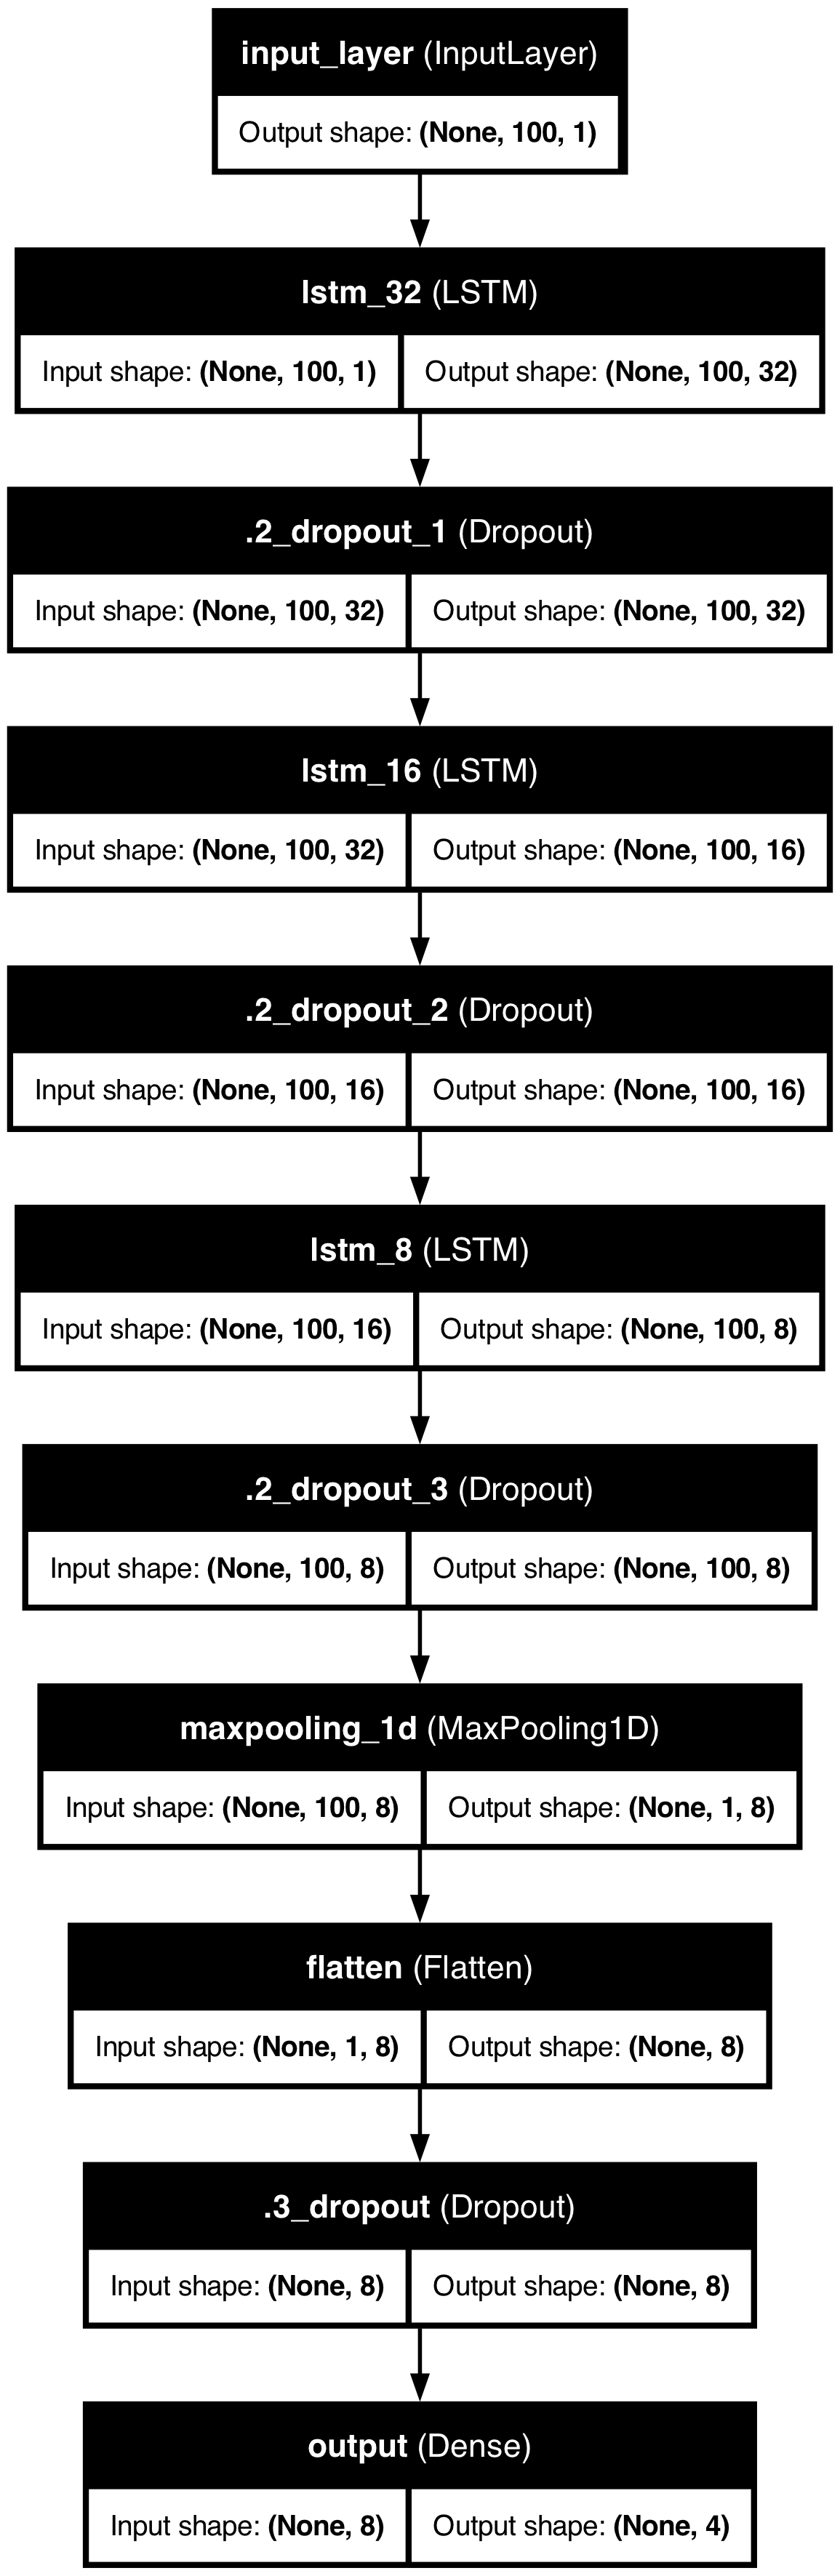
\includegraphics[width=\textwidth]{plotsss/rnn_ts.png}
%         \captionof{figure}{RNN model architecture}
%         \label{fig:rnn_model}
%     \end{minipage}
% \end{figure}

Figure~\ref{fig:loss_acc} shows the training and validation loss and accuracy
over epochs.
\begin{figure}[H]
    \centering
    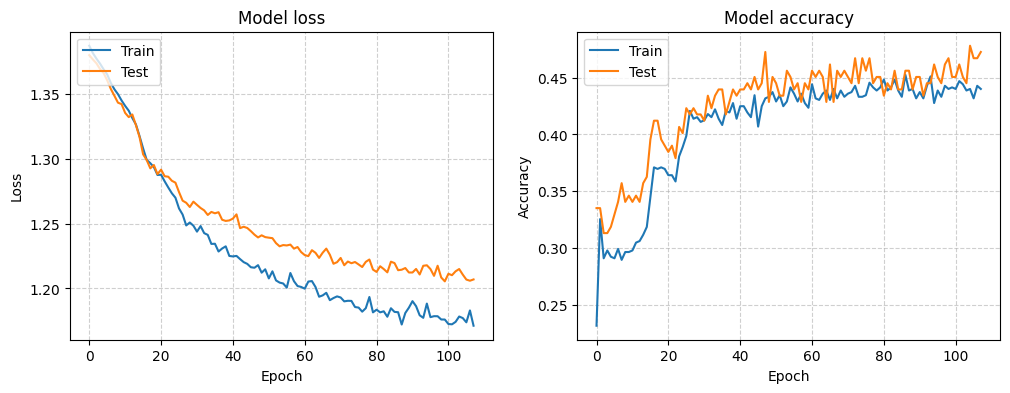
\includegraphics[width=0.9\textwidth]{plotsss/ts_loss_acc.png}
    \caption{Training and validation loss and accuracy over epochs}
    \label{fig:loss_acc}
\end{figure}

The loss graph shows a steady decrease about halfway through training.
At this point, it records a sharp decrease in loss, followed by another
period of steady decrease.


\begin{figure}[H]
    \centering
    \begin{minipage}{0.6\textwidth}
        Figure~\ref{fig:cm_rnn} shows the confusion matrix for the RNN
        model on the test set.
    \end{minipage}
    \hfill
    \begin{minipage}{0.35\textwidth}
        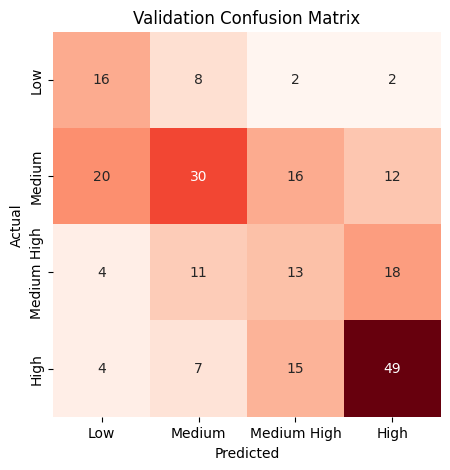
\includegraphics[width=1\textwidth]{plotsss/rnn_cm.png}
        \caption{Confusion matrix for the RNN model on the test set}
        \label{fig:cm_rnn}
    \end{minipage}
\end{figure}